\begin{figure}[h]
    \centering
    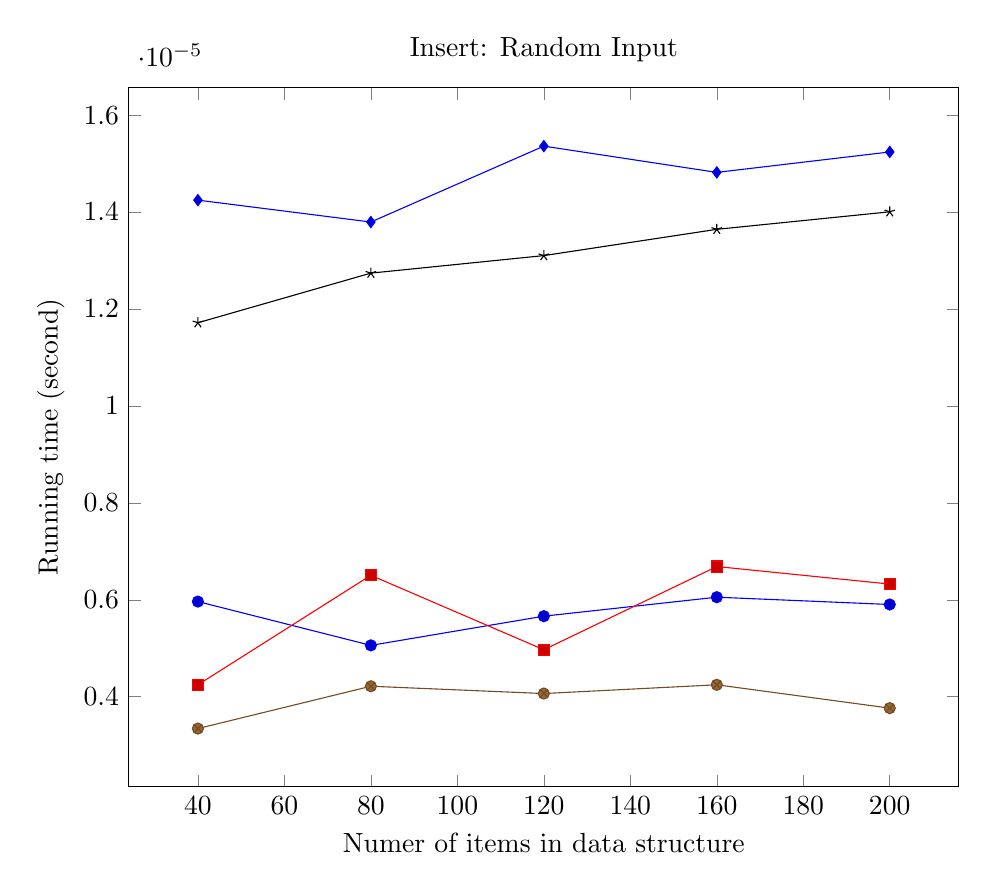
\begin{tikzpicture}
        \begin{axis}[
            xlabel={Numer of items in data structure},
            ylabel={Running time (second)},
            title={Insert: Random Input},
            width=\textwidth
        ]
		\addplot coordinates {
			(200, 5.903036600329869e-06)
			(160, 6.053624268531621e-06)
			(120, 5.662096330993905e-06)
			(80, 5.059745657476355e-06)
			(40, 5.9632716677526785e-06)
		};
		\addplot coordinates {
			(200, 6.324682071934263e-06)
			(160, 6.686092475760575e-06)
			(120, 4.969393056342142e-06)
			(80, 6.505387273847419e-06)
			(40, 4.246572247978974e-06)
		};
		\addplot coordinates {
			(200, 3.7646917093070444e-06)
			(160, 4.246572248334246e-06)
			(120, 4.065867046065818e-06)
			(80, 4.216454714622841e-06)
			(40, 3.343046238057923e-06)
		};
		\addplot coordinates {
			(200, 1.4004653159105374e-05)
			(160, 1.364324275492379e-05)
			(120, 1.3101127148473779e-05)
			(80, 1.2739716744292196e-05)
			(40, 1.1715720599525526e-05)
		};
		\addplot coordinates {
			(200, 1.5239472039851876e-05)
			(160, 1.4817826568247482e-05)
			(120, 1.5359942174342223e-05)
			(80, 1.3793830423125541e-05)
			(40, 1.4245593428441339e-05)
		};
        \legend{}
        \end{axis}
    \end{tikzpicture}
    \caption{Average of 0 operations, benchmarked every 0, starting at 0.}
\end{figure}